\documentclass[12pt]{article}

\usepackage[french]{babel}
\usepackage[utf8]{inputenc}  
\usepackage[T1]{fontenc}
\usepackage[left=2.5cm,right=2.5cm,top=3cm,bottom=2.65cm]{geometry}
\usepackage{amsmath,amssymb,amsfonts}
\usepackage{algorithm}
\usepackage{algpseudocode}
\usepackage{graphicx}
\usepackage{caption}
\usepackage{tikz}

\graphicspath{{ims/}}

\title{
	Distributed Systems\\
	\textbf{Building a distributed neural network}\\
	Report
}
\author{
	Yoann Coudert-\,-Osmont
}

\begin{document}
	
\maketitle

\section{Introduction}

In this project a neural network for distributed systems has been implemented. We use an architecture with fully connected layers. Each neuron of the network is a single process which communicate with its in-neurons and out-neurons. The user can spawn a monitor which will create the network an manage it.

\paragraph{How to use the code}
The source code is in the folder \verb|src|. There are two files which were given to us at the beginning of the project (\verb|dataframe.erl| and \verb|utils.erl|) to make easier the use of 2d arrays and to read CSV files.
\begin{itemize}
	\item The file \verb|network.erl| contains functions executed by neurons and a function to spawn a network.
	\item The file \verb|monitor.erl| contains the code of the monitor.
	\item The file \verb|testing.erl| allows to test the efficiency of different architectures of neural networks.
\end{itemize}
The folder \verb|testing| contains some Python script to plot some graphics which are in this report. The folder \verb|data| contains two data-sets in CSV format. \\
To execute the code you can use:
\begin{itemize}
	\item \verb|make network| to test feed-forward, feed-backward and interruption of these scenarios. More precisely it tests the interruption of a feed-forward scenario at the begging. Next it try to make the network output 1 on the input (0.5, 0.4). It print at each step two lines with \verb|res = done| for the feed-backward scenario and \verb|res = <a float>| for the result of the feed-forward scenario. This result should increase. At the end it tries to interrupt a feed-backward scenario.
	\item \verb|make monitor| to test the monitor which tests backpropagation algorithm on the data-set in the file \verb|training_set.csv|.
	\item \verb=make testing | python3 testing/stats.py= to plot some graphs about the efficiency of different neural network architectures.
\end{itemize}

\paragraph{Parameters}
At the beginning of the file \verb|src/network.erl| there is a section parameters in which you can:
\begin{itemize}
	\item Choose the time before re-sending a message when no ack has been received.
	\item Choose the learning rate.
	\item Activate the verbose mode.
	\item Choose the probability of failure when sending a message between two neurons.
\end{itemize}

\section{Network deployment}

I spawn all neurons on the same node. I didn't implemented a way to spawn layers on different nodes. The function that spawn a network is \verb|network:neural_network/2|. the first parameter is a list of the sizes of each layer. The second is the PID of the monitor with which output and input neurons will communicate. I use a trick which consist in spawning a new input neurons before the true layer of inputs neurons. This new neurons will have a list of values to feed to the true input layer in feed-forward scenario.

\begin{figure}[h]
	\centering
	\begin{tikzpicture}[every node/.style={minimum size=0.75cm}]
		\node[fill=blue, draw, circle, opacity=0.5] (a) at (0, 0) {};
		
		\node[fill=green, draw, circle, opacity=0.5] (b) at (2.5, -1.4) {};
		\node[fill=green, draw, circle, opacity=0.5] (c) at (2.5, 0) {};
		\node[fill=green, draw, circle, opacity=0.5] (d) at (2.5, 1.4) {};
		
		\node[fill=gray, draw, circle, opacity=0.5] (e) at (5, -0.7) {};
		\node[fill=gray, draw, circle, opacity=0.5] (f) at (5, 0.7) {};
		
		\node[fill=gray, draw, circle, opacity=0.5] (g) at (7.5, -0.7) {};
		\node[fill=gray, draw, circle, opacity=0.5] (h) at (7.5, 0.7) {};
		
		\node[fill=red, draw, circle, opacity=0.5] (i) at (10, 0) {};
		
		\node[fill=black, draw, circle, opacity=0.5] (j) at (5, 3) {};
		\draw[<->] (a) edge[bend left] (j);
		\draw[<->] (i) edge[bend right] (j);
		
		\node at (6.25, -1.8) {\small Hidden layers};
		\node at (2.5, -2.4) {\small Input layer};
		\node at (-0.3, -1) {\small Input neuron};
		\node at (10.3, -1) {\small Output neuron};
		\node at (5, 3.75) {\small Monitor};
		
		\draw[<->] (a) -- (b);
		\draw[<->] (a) -- (c);
		\draw[<->] (a) -- (d);
		
		\draw[<->] (b) -- (e);
		\draw[<->] (b) -- (f);
		\draw[<->] (c) -- (e);
		\draw[<->] (c) -- (f);
		\draw[<->] (d) -- (e);
		\draw[<->] (d) -- (f);
		
		\draw[<->] (e) -- (g);
		\draw[<->] (e) -- (h);
		\draw[<->] (f) -- (g);
		\draw[<->] (f) -- (h);
		
		\draw[<->] (g) -- (i);
		\draw[<->] (h) -- (i);
	\end{tikzpicture}
	\captionsetup{justification=centering}
	\caption{All processes spawned and links between them. The first argument of
		\texttt{network:neural\_network/2} was \texttt{[3, 2, 2, 1]}. }
	\label{net}
\end{figure}

Layers are spawn one after the other starting from the layer of the output neuron. Neurons are spawn with their out-layer in parameter then they are waiting for a message containing their in-layer. When the in-layer is spawned we send it.

I have three different functions for the neuron. A function for hidden neurons and for the neurons of the true input layer, a function for the input neuron and a function for the output neuron.

\section{Feed-forward and feed-backward scenarios}

\paragraph{Weights and Bias}
As proposed weights and bias are initialized with random values $\sim \mathcal{N}(0, 1)$. I created a record \verb|hd| that contains data of hidden neurons (When I say hidden neuron, I include neurons of the input layer. I only distinguish the input neuron and the output neuron from other neurons). In this record I store the weights of connections toward the out-layer (i.e. the values $w_{ij}^{l+1}$ for the neuron $j$ of the layer $l$ using the notations of the subject). I preferred store these weights instead of weights of the connections with in-layer $w_{jk}^l$ as proposed in the subject because it allow us to avoid the need to store the values of in-neuron to update weights during the feed-backward scenario. In fact we have:
$$ w_{ij}^{l+1} \gets w_{ij}^{l+1} - \eta a_j^l \delta_i^{l+1} $$
Then the $j$-th neuron of the $l$-th layer has to send weighted values during feed-forward scenario (i.e. it sends $w_{ij}^{l+1} a_j^l$ to the $i$-th neuron of the $(l+1)$-th layer).

I also store the bias $b_j^l$ in \verb|hd|. As neurons of the input layer should not have a bias, the record also have a value \verb|input_layer| which is \verb|true| if and only if the neuron is a neuron of the input layer. When this value is \verb|true|, the bias $b$ is forced to be 0.

Furthermore the output neuron stores its own bias.

\paragraph{Communications}
I created another record \verb|com| for communications. The three parameters of the hidden neuron function are a record \verb|hd| containing the data of the neuron, and two record \verb|com|, one for the communication of the feed-forward scenario and another for the communication of the feed-backward scenario.

Now I will explain how communications works in the case of feed-forward scenario. I use the idea of the alternative-bit algorithm. In the \verb|com| record I have the following values:
\begin{itemize}
	\item \verb|rcv|, an array which store a bit for all neuron from which we will receive messages (i.e. neurons of the in-layer in the case of feed-forward scenario).
	\item \verb|send|, an array which store a bit for all neuron to which we will send messages (i.e. neurons of the out-layer in the case of feed-forward scenario).
	\item \verb|miss_rcv|, the number of messages that we need to receive.
	\item \verb|miss_send|, the number of ack that we need to receive.
	\item \verb|timeout|, the time in nano-seconds of the last message sent.
	\item \verb|bit|, the alternative-bit that represent the state of the communication.
\end{itemize}
The two arrays \verb|rcv| and \verb|send| are initialized with zeros. \verb|bit| is also initialized to zero. Finally the first state of a neuron is waiting for data so \verb|miss_rcv| is initialized to the length of \verb|rcv| (\verb|size(rcv)|) and \verb|miss_send| is initialized to zero.

We can describe the protocol with three labels. Two labels for receiving messages and one label for re-sending messages for which the ack has not been received (\figurename~\ref{proto}). The pseudo-code is given for feed-forward scenario but it is almost the same for feed-backward scenario expect that we send values to in-neurons, receive values from out-neuron and communicate $\delta_j^l$ instead of $w_{ij}^{l+1} a_j^l$.

\newpage

\begin{figure}[t]
	\fbox{\parbox{\linewidth}{
	\texttt{RCV\_ACK: [receive <forward, ack, i, b>]} \\
	. \qquad \texttt{if b == bit and send[i] == bit:} \\
	. \qquad \qquad \texttt{miss\_send = miss\_send - 1} \\
	. \qquad \qquad \texttt{send[i] = (bit + 1) mod 2} \\
	. \qquad \qquad \texttt{if miss\_send == 0:} \\
	. \qquad \qquad \qquad \texttt{bit = (bit + 1) mod 2} \\
	. \qquad \qquad \qquad \texttt{miss\_rcv = size(rcv)} \\
	\\
	\texttt{RCV\_VAL: [receive <forward,} $w_{jk}^l a_k^{l-1}$\texttt{, k, b>]} \\
	. \qquad \texttt{if b == bit or miss\_send == 0:} \\
	. \qquad \qquad \texttt{send <forward, ack, j, b> to k-th in-neuron} \\
	. \qquad \texttt{if b == bit and rcv[k] == bit:} \\
	. \qquad \qquad \texttt{miss\_rcv = miss\_rcv - 1} \\
	. \qquad \qquad \texttt{rcv[k] = (bit + 1) mod 2} \\
	. \qquad \qquad \texttt{update} $a_j^l$ \texttt{thanks to} $w_{jk}^l a_k^{l-1}$ \\
	. \qquad \qquad \texttt{if miss\_rcv == 0:} \\
	. \qquad \qquad \qquad $\forall$ \texttt{i, send <forward,} $w_{ij}^{l+1} a_j^l$\texttt{, j, b> to i-th out-neuron} \\
	. \qquad \qquad \qquad \texttt{miss\_send = size(send)} \\
	. \qquad \qquad \qquad \texttt{timeout = get\_Time()} \\
	\\
	\texttt{RE-SEND: [miss\_send > 0 and get\_Time() - timeout > DT]} \\
	. \qquad $\forall$ \texttt{i, if send[i] == bit:} \\
	. \qquad \qquad \texttt{send <forward,} $w_{ij}^{l+1} a_j^l$\texttt{, j, b> to i-th out-neuron} \\
	. \qquad \texttt{timeout = get\_Time()} \\
	}}
	\caption{Protocol of communication in the case of feed-forward scenario}
	\label{proto}
\end{figure}

This is how hidden-neurons work but we need to initiate the feed-forward scenario. For this the monitor sends the array containing all input values to the input neuron (in red in the \figurename~\ref{net}). This input neuron sends values of the array to all neurons in the true input layer (in green in the \figurename~\ref{net}) until it receive ack from everyone. Finally when output neuron has received all his input values, he computes his value and send it to the monitor. In feed-backward scenario, when the input neuron has received all errors of all neurons of the true input layer it sends a message saying that the backprop is done to the monitor.

\paragraph{Results} With this protocol neurons won't wait if a message is lost. You can modify the \verb|err_prob| parameter in the \verb|src/network.erl| file to add a probability of failure when sending a message. Then you can test that everything works with \verb|make network|. To see all messages you can set \verb|verbose| to \verb|true|. You will see all messages during the process. You can also look at the impact of the \verb|dt| parameter which is the time before re-sending a message. I set it to 20ms but if we decrease this value the execution time reduces when the probability of failure is non-null. The \figurename~\ref{err_prob} shows the impact of the \verb|err_prob| parameter on execution time.

\begin{figure}
	\centering
	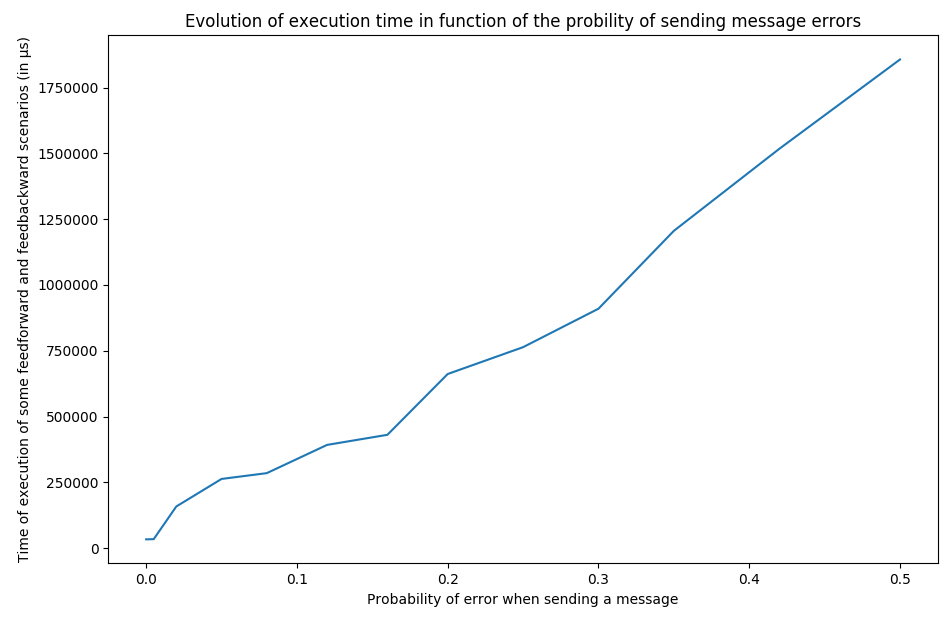
\includegraphics[scale=0.6]{prob_error.png}
	\captionsetup{justification=centering}
	\caption{Evolution of execution time in function of the probability of error in the sending of messages}
	\label{err_prob}
\end{figure}

\section{Interruptions and Shutdown}

\paragraph{Interruption}
Again, interruption of feed-backward scenario is very similar to the interruption of feed-forward scenario so I will only present the interruption of feed-forward scenario. As the feed-forward scenario starts in the input neuron and ends in the output neuron if the interruption starts in the input neuron maybe the wave of interruption won't reach the wave of feed-forward before the scenario is finished. So we start the interruption in the output neuron.

I first thought that I could only reinitialize the \verb|com| record to make neurons forget their previous messages. But by doing this certain neurons after being reset, could receive messages from neurons that had not been reinitialized yet and then they thought a new wave has begun. That's why I decided to use two passes as illustrated in \figurename~\ref{inter}. The first pass interrupt neurons in the sense that when they are interrupted they ignore messages of feed-forward scenario and they stop send messages. When the input neuron receive the interruption message it start a new pass which reset the \verb|com| record of neurons. In this way, when neurons are reset they don't receive messages because other neurons are either interrupted or reset.

To limit the number of messages, only the first neuron of each layer sends the interruption message to the next layer.

\paragraph{Shutdown}
You can also send a message \verb|shutdown| to the monitor that will send it to the input neuron and then the input neuron send it to the next layer and the first neuron of each layer transmit the message to its out-neurons. After receiving a message \verb|shutdown|, a process finish. Like this you can properly stop all processes.

\begin{figure}[h]
	\centering
	\begin{tikzpicture}[every node/.style={minimum size=0.75cm}, >={latex}, scale=0.9]
	\node[fill=blue, draw, circle, opacity=0.5] (a) at (0, 0) {};
	
	\node[fill=green, draw, circle, opacity=0.5] (b) at (2.5, -1.4) {};
	\node[fill=green, draw, circle, opacity=0.5] (c) at (2.5, 0) {};
	\node at (2.5, 0) {$\bigotimes$};
	\node[fill=green, draw, circle, opacity=0.5] (d) at (2.5, 1.4) {};
	
	\node[fill=gray, draw, circle, opacity=0.5] (e) at (5, -0.7) {};
	\node at (5, -0.7) {$\bigotimes$};
	\node[fill=gray, draw, circle, opacity=0.5] (f) at (5, 0.7) {};
	\node at (5, 0.7) {$\bigotimes$};
	
	\node[fill=gray, draw, circle, opacity=0.5] (g) at (7.5, -0.7) {};
	\node at (7.5, -0.7) {$\bigotimes$};
	\node[fill=gray, draw, circle, opacity=0.5] (h) at (7.5, 0.7) {};
	\node at (7.5, 0.7) {$\bigotimes$};
	
	\node[fill=red, draw, circle, opacity=0.5] (i) at (10, 0) {};
	\node at (10, 0) {$\bigotimes$};
	
	\node[fill=black, draw, circle, opacity=0.5] (j) at (5, 2.8) {};
	
	\node at (-0.3, -1) {\small Input neuron};
	\node at (10.3, -1) {\small Output neuron};
	\node at (5, 3.55) {\small Monitor};
	
	\node[draw,rectangle] at (0.1, 3.4) {$\bigotimes$: interrupted};
	
	\draw[->, purple, thick] (j) edge[bend left] (i);
	\draw[->, purple, thick] (i) -- (g);
	\draw[->, purple, thick] (i) -- (h);
	\draw[->, purple, thick] (h) -- (e);
	\draw[->, purple, thick] (h) -- (f);
	\draw[->, purple, thick, opacity=0.3] (f) -- (b);
	\draw[->, purple, thick] (f) -- (c);
	\draw[->, purple, thick, opacity=0.3] (f) -- (d);
	\draw[->, purple, thick, opacity=0.3] (d) -- (a);
	\end{tikzpicture}
	\begin{tikzpicture}[every node/.style={minimum size=0.75cm}, >={latex}, scale=0.9]
	\node[fill=blue, draw, circle, opacity=0.5] (a) at (0, 0) {};
	\node at (0, 0) {$\bigcirc$};
	
	\node[fill=green, draw, circle, opacity=0.5] (b) at (2.5, -1.4) {};
	\node at (2.5, -1.4) {$\bigcirc$};
	\node[fill=green, draw, circle, opacity=0.5] (c) at (2.5, 0) {};
	\node at (2.5, 0) {$\bigcirc$};
	\node[fill=green, draw, circle, opacity=0.5] (d) at (2.5, 1.4) {};
	\node at (2.5, 1.4) {$\bigcirc$};
	
	\node[fill=gray, draw, circle, opacity=0.5] (e) at (5, -0.7) {};
	\node at (5, -0.7) {$\bigcirc$};
	\node[fill=gray, draw, circle, opacity=0.5] (f) at (5, 0.7) {};
	\node at (5, 0.7) {$\bigcirc$};
	
	\node[fill=gray, draw, circle, opacity=0.5] (g) at (7.5, -0.7) {};
	\node at (7.5, -0.7) {$\bigotimes$};
	\node[fill=gray, draw, circle, opacity=0.5] (h) at (7.5, 0.7) {};
	\node at (7.5, 0.7) {$\bigotimes$};
	
	\node[fill=red, draw, circle, opacity=0.5] (i) at (10, 0) {};
	\node at (10, 0) {$\bigotimes$};
	
	\node[fill=black, draw, circle, opacity=0.5] (j) at (5, 2.8) {};
	
	\node at (-0.3, -1) {\small Input neuron};
	\node at (10.3, -1) {\small Output neuron};
	\node at (5, 3.55) {\small Monitor};
	
	\node[draw,rectangle] at (0.1, 3.4) {$\bigcirc$: reinitialized};
	
	\draw[->, brown, thick] (a) -- (b);
	\draw[->, brown, thick] (a) -- (c);
	\draw[->, brown, thick] (a) -- (d);
	\draw[->, brown, thick] (d) -- (e);
	\draw[->, brown, thick] (d) -- (f);
	\draw[->, brown, thick, opacity=0.3] (f) -- (g);
	\draw[->, brown, thick, opacity=0.3] (f) -- (h);
	\draw[->, brown, thick, opacity=0.3] (h) -- (i);
	\end{tikzpicture}
	\captionsetup{justification=centering}
	\caption{Interruption of a feed-forward scenario.}
	\label{inter}
\end{figure}

\section{Monitor}

My monitor is very simple. I have nothing particular to say about it. I have only implemented what we were asked to implement from question a) to question f). I didn't implement a mechanism to detect neurons failure and a way to re-spawn neurons. The function \verb|test| in the file \verb|src/monitor.erl| is an example to learn to use the monitor. You can run this function with \verb|make monitor|.

\section{Testing}

\begin{figure}
	\centering
	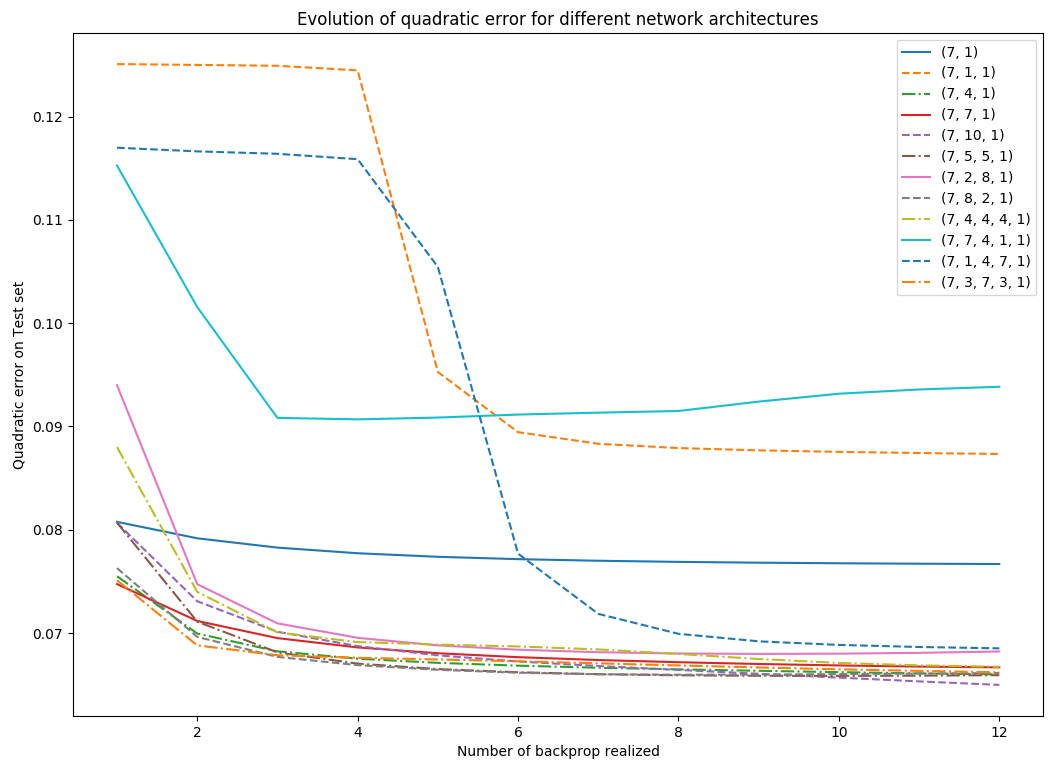
\includegraphics[scale=0.5]{error.png}
	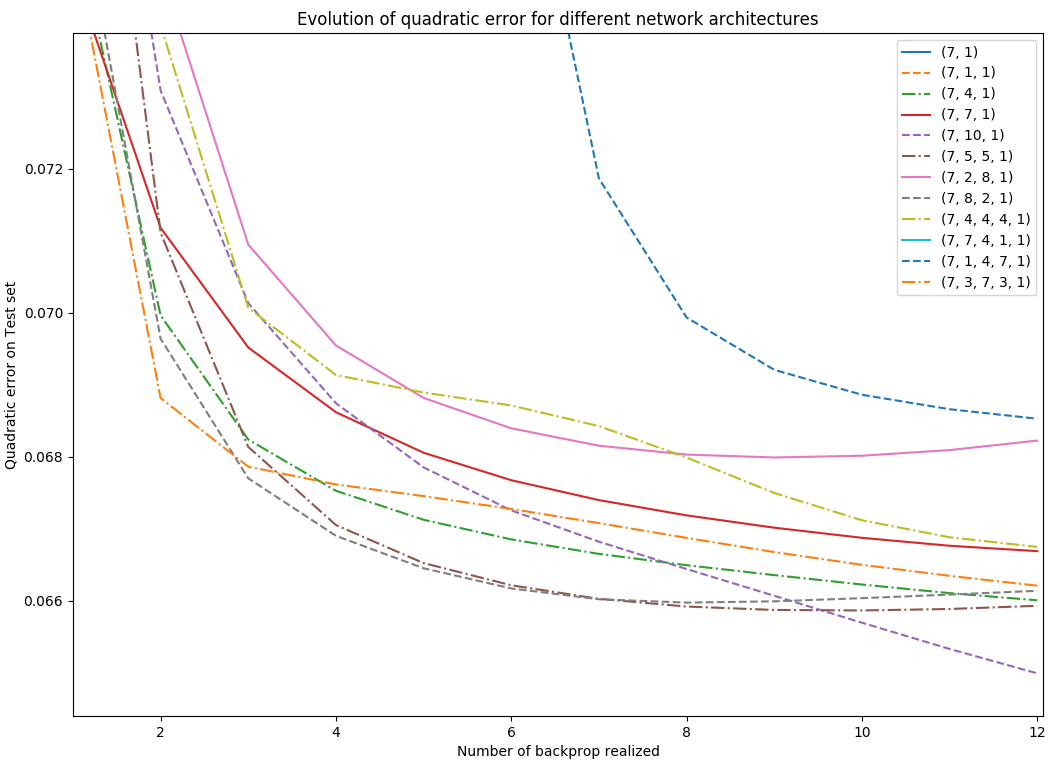
\includegraphics[scale=0.5]{error_zoom.png}
	\captionsetup{justification=centering}
	\caption{Evolution of quadratic error for different network architectures}
	\label{err}
\end{figure}

I tried different architectures in the file \verb|src/testing.erl|. You can run this script with \verb|make testing| and it will print some stats that can be plot thanks to the Python3 script \verb|testing/stats.py|. I experimented the influence of the network size on the evolution of the error on the test set (as proposed I separated the set in a train set and a test set with proportion 70/30\%). I obtained the graphic in the \figurename~\ref{err}. The tuples in the legend give the number of neurons in each layer. I measured also the time of execution and I obtained the graphic in the \figurename~\ref{time}. The orange dots in this graphics have a height proportional to the numbers of parameters to learn in the network architecture. As we can see the number of parameters seems to be correlated with the execution time.

\begin{figure}
	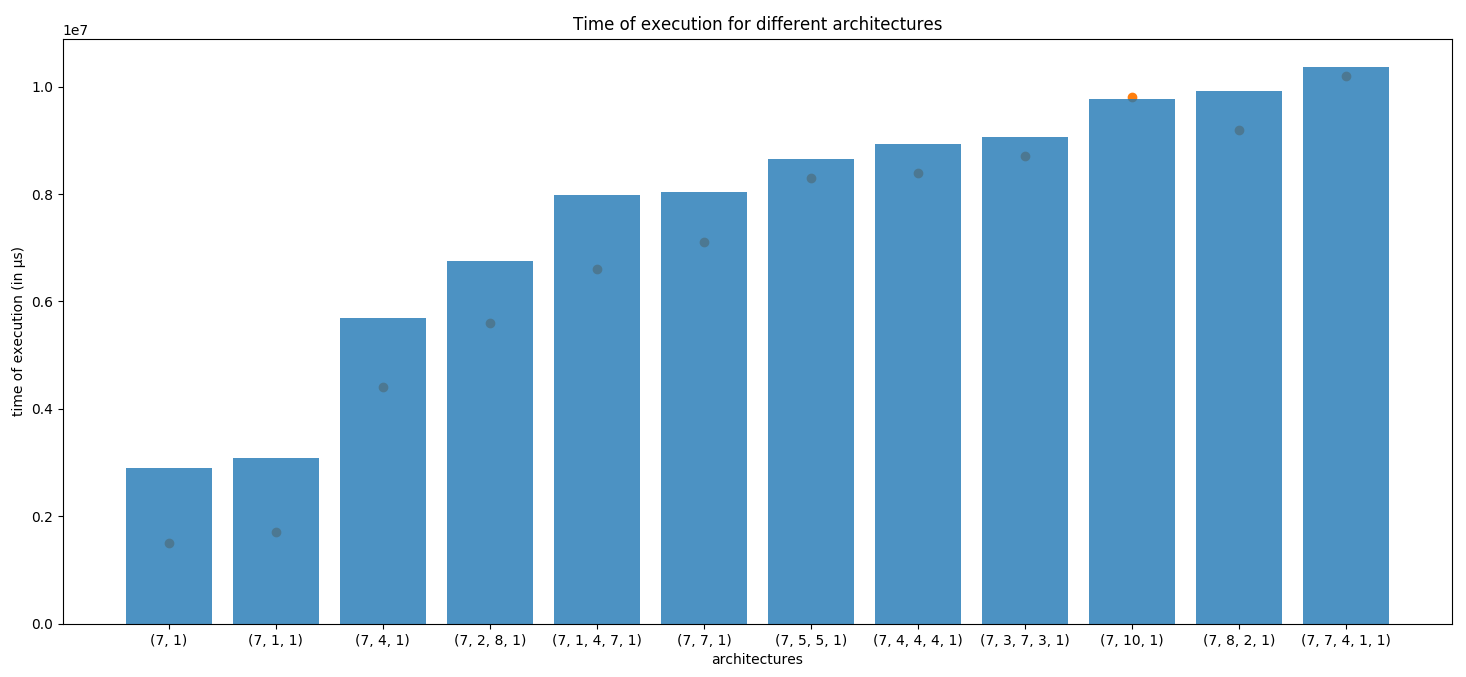
\includegraphics[scale=0.45]{time.png}
	\caption{Time of execution for different architectures}
	\label{time}
\end{figure}

\section{Discussion}

I don't think that it is a good idea to distribute a neural network in this way. In fact computations made by each neurons are very simple. Then what is most time-consuming is communication and not computations in what I have done. We need to make processes make more computations before sending messages. In this way, the communication won't be a time-consuming problem. 

Then another way to distribute a neural network is to spawn different processes where each process has a copy of the whole network. Then we can split the training set and give a subset to each process that will perform back-propagation on the training subset. When each process has finish they can send their new parameters to a server that will combined results of all processes to create new optimized parameters and send it to all processes. Then we restart, we split the training set, ... 

\end{document}